\documentclass[A4,11pt]{article}


\usepackage{url,graphicx,array,authblk}
\usepackage[usenames,dvipsnames]{color}

\usepackage{graphicx,setspace}
\usepackage[margin=1in]{geometry}
\usepackage[utf8]{inputenc}
\usepackage{multirow}
\usepackage{natbib}
\usepackage{amsmath,amssymb,mathtools,amsthm}
\DeclarePairedDelimiter{\ceil}{\lceil}{\rceil}
\DeclarePairedDelimiter{\floor}{\lfloor}{\rfloor}
\usepackage[title]{appendix}
\newcommand{\HRule}{\rule{\linewidth}{0.35mm}}

\makeatletter

\makeatother

\usepackage{placeins}

\usepackage{listings}
\usepackage{float,mdwlist,enumitem}
\usepackage{footmisc}

\newcolumntype{C}[1]{>{\centering\arraybackslash}p{#1}} 
\newcolumntype{L}[1]{>{\raggedright\arraybackslash}p{#1}} 
\newcolumntype{R}[1]{>{\raggedleft\arraybackslash}p{#1}} 
\newlength\interColSepSmall
\newlength\interColSepLarge
\setlength{\interColSepSmall}{0.2em}
\setlength{\interColSepLarge}{0.4em}

\setlength{\parindent}{0em}
\setlength{\parskip}{0.4em}

\usepackage{booktabs}
\usepackage[colorlinks = true,
            linkcolor =black,
            urlcolor  = black,
            citecolor = black,
            anchorcolor = black]{hyperref}


\usepackage{siunitx}
\usepackage{dcolumn}
\newcolumntype{e}[1]{D{.}{.}{#1}}
\newcommand{\muc}[2]{\multicolumn{1}{C{#1}}{#2}}
\newcommand{\mul}[2]{\multicolumn{1}{L{#1}}{#2}}
\newcommand{\suc}[1]{\multicolumn{1}{c}{#1}}
\newcommand{\mucThree}[2]{\multicolumn{3}{C{#1}}{#2}}
\newcommand{\mulTen}[2]{\multicolumn{10}{L{#1}}{#2}}


% Natbib setup for author-year style
\usepackage{natbib}
 \bibpunct[, ]{(}{)}{,}{a}{}{,}%
 \def\bibfont{\small}%
 \def\bibsep{\smallskipamount}%
 \def\bibhang{24pt}%
 \def\newblock{\ }%
 \def\BIBand{and}%

\newcommand{\dyad}{dyad}
\usepackage{tikz}
\usetikzlibrary{shapes.geometric, matrix, positioning, calc, intersections}
\usetikzlibrary{patterns}
\usetikzlibrary{decorations.pathmorphing}
\usepackage{pgfplots,pgfmath,xcolor}



\usetikzlibrary{arrows,positioning} 

\usetikzlibrary {arrows.meta}

\definecolor{darkblue}{rgb}{0.3,0.5,1}

\makeatletter
\pgfmathdeclarefunction{erf}{1}{%
  \begingroup
    \pgfmathparse{#1 > 0 ? 1 : -1}%
    \edef\sign{\pgfmathresult}%
    \pgfmathparse{abs(#1)}%
    \edef\x{\pgfmathresult}%
    \pgfmathparse{1/(1+0.3275911*\x)}%
    \edef\t{\pgfmathresult}%
    \pgfmathparse{%
      1 - (((((1.061405429*\t -1.453152027)*\t) + 1.421413741)*\t 
      -0.284496736)*\t + 0.254829592)*\t*exp(-(\x*\x))}%
    \edef\y{\pgfmathresult}%
    \pgfmathparse{(\sign)*\y}%
    \pgfmath@smuggleone\pgfmathresult%
  \endgroup
}
\makeatother

\tikzset{
mainnode/.style={
    rectangle,
    draw=black,
    fill=white,
    thick,
    minimum size=5mm,
    text width=40mm,
    text height = 10pt,
    text depth = 3pt
},
ovalbignode/.style={
    ellipse,
    draw=black,
    fill=white,
    thick,
    minimum size=40mm,
    text width=50mm,
    fill opacity=.2,
    text opacity=1
},
papernode/.style={
    rectangle,
    minimum size=5mm,
    text width=68mm,
    font=\normalfont
},
decisionnode/.style={
    diamond, 
    draw=black, 
    thick, 
    text centered,
    minimum width=15mm,
    minimum height=15mm, 
    inner sep=0pt
},    
align=center
}

\newcommand{\nodeLabel}[2]{\node[labelnode] [above right=-0.15cm and -0.3cm of #1] {#2};}

\newcommand{\checkbox}{\tikz\draw (0,0) rectangle (0.3,0.3);}

\newcommand{\radiobutton}{\tikz\draw (0,0) circle (0.15);}

\usetikzlibrary{positioning, shapes, arrows.meta}


%%%%%%%%%%%%%%%%
\begin{document}
%%%%%%%%%%%%%%%%

\subsection*{1. Contact Information}
% Note that the experimenter must be a researcher with TUM (PhD student or better). The experimenter must run the experiment personally.
\begin{enumerate}
\item Mrunal Mohadikar - Doctoral student in Supply Chain Management, TUM School of Management, Technical University of Munich\\ \href{mailto:mrunal.mohadikar@tum.de}{(mrunal.mohadikar@tum.de)}, +49 713126418831
\item Prof. Dr. David Wuttke - Assistant Professor of Supply Chain Management, TUM School of Management, Technical University of Munich\\ \href{mailto:david.wuttke@tum.de}{(david.wuttke@tum.de)}, +49 713126418804
\item Prof. Dr. Enno Siemsen - Professor of Operations and Information Management, Wisconsin School of Business, University of Wisconsin-Madison\\ 
\href{mailto:esiemsen@wisc.edu}{(esiemsen@wisc.edu)}
\end{enumerate}

\subsection*{2. Title of the Experiment} 
% The title is for internal use and is supposed to characterize the experiment for people unfamiliar with it.
Augmented Reality in field-based service operations: How the dyad formation is affected?

\subsection*{3. Description of the Experiment}
% It must be clear from the description that the experiment complies with experimenTUM’s policies.
%The goal of the experiment is to find out how a dyad (pair) of subjects performs when the subject is working repeatedly with the same partner (dedicated), and when the partner is different (random). The experiment also looks at how the performance is affected when the dyad works remotely, and together on-site. For this, a real-effort experiment will be conducted in two parts - one with the use of Augmented Reality and one without. 

The objective of the experiment is to evaluate how Augmented Reality (AR) technology impacts the performance dynamics between technician-expert dyads in field-based service operations. This study specifically investigates the role of AR in modifying the effectiveness of dedicated and random dyad formations. Dedicated dyads consist of a fixed technician and expert pair that consistently work together, while random dyads are formed by pairing technicians with any available expert. The experiment aims to determine whether AR enhances or limits the performance benefits typically associated with each dyad type by improving problem-solving capabilities, learning opportunities, and communication efficiency.

In deploying AR technologies, such as smart glasses that overlay real-time visual and textual information, this research hypothesizes potential shifts in operational advantages. It posits that AR could either amplify the benefits of random dyads by introducing varied perspectives and creative problem-solving or could strengthen dedicated dyads by making communication more seamless and collaboration more effective. The study explores these hypotheses by examining the interactions within these dyads during service repair tasks, both in remote and on-site settings, to understand better how AR can be strategically utilized to enhance service management practices in various industries.

The experimental design involves a controlled setup where the complexity of tasks (whether simple or complex) and the proximity of dyad members (whether collaborating on-site or remotely) are varied to assess their impact on the performance of service repairs. The experiment aims to provide evidence on how AR can be optimally employed to refine the efficiency and effectiveness of technician-expert collaborations in field services by systematically evaluating the performance outcomes of different dyad configurations under these varied conditions. This research could potentially redefine strategies within service operations, paving the way for more innovative and effective use of technology in complex environments.

The experiment will follow a between-subject design, with each subject assigned to one of two conditions in each part---either a dedicated or random condition. Each part will have 120 student participants, thus 240 participants in total. These students will be organized into ten sessions per part, each session accommodating 12 subjects. Each session, unknown to the participants, will either be a random dyad condition or a dedicated dyad condition. Within each session, 6 students will be randomly assigned the role of technicians, while the remaining 6 will assume the role of experts. Each technician student will be randomly paired with an expert student in their condition.

The student dyads will have to repair six faulty microcontroller circuit boards. For this, the students will be provided with comprehensive guidelines outlining the basics of circuit boards and electrical components. In addition, students assigned as experts will be provided with supplementary instructional materials in the form of a video guide focusing on electrical components and will be provided with trial tasks to work on. For sessions with AR, the technicians will receive further training on using the AR device.

To illustrate the specific task, we created a video that can be accessed using the following link:

\url{https://syncandshare.lrz.de/getlink/fiBzutdPjNKR3ed68Ubksz/4.Participants_View.mp4}

Lastly, the students will receive a fixed payment for their participation, supplemented by an additional payment based on the collaborative performance of the dyad with which they were engaged. Figure~\ref{fig:experiment_flow} depicts the flow of the experiment for a session.

\begin{figure}[h]
    \centering
    \begin{tikzpicture}
         \node (student) [mainnode,text centered] {Subject enters};
         
         \node (information) [mainnode,text centered, text width=7cm, below=0.7cm of student] {Informational video on VR headset};
         \node (sickness) [decisionnode,text centered, below=0.5cm of information] {Motion\\sickness?};
%         \node[papernode] at (6.5,-3.5) {\small{Note: Only applicable for AR sessions.}};
         \node[papernode] at (3,-5) {\small{Yes}};
         \node[papernode] at (-0.25,-4.6) {\small{No}};
         
         \node (technician) [mainnode,text centered, below left=2.5cm and 2cm of sickness] {Technician};
         \node (expert) [mainnode,text centered, right=6cm of technician] {Expert};
         \node[papernode] at (0,-5.9) {\small{Random allocation\\to have equal number of technician and expert}};
         \node (ar_training) [mainnode,text centered, below=0.7cm of technician] {AR training};
         \node (expert_training) [mainnode,text centered, below=0.7cm of expert] {Expert training};
         \node (manipulation) [mainnode,text centered, below right=1cm and 1cm of ar_training] {Manipulation check};
         %\node[papernode] at (0,-10.9) {\small{Random assignment}};
         \node (dyad) [decisionnode,text centered, below=0.5cm of manipulation] {Dyad\\assignment\\\small{a/c session}};
         \node (dedicated_dyad) [mainnode,text centered, below left=1cm and 1cm of dyad] {\textbf{Dedicated \dyad}};
         \node (random_dyad) [mainnode,text centered, right=4cm of dedicated_dyad] {\textbf{Random \dyad}};

         %\node[papernode] at (1.4,-13.1) {\small{Allocation as per session}};
         
         \node (task) [mainnode,text centered, text width=5.5cm, minimum height=2cm, below=2cm of dyad, anchor=north, text height=0cm, text depth=1cm] {1 & & 2 & & 3 & & 4 & \;\;\;\;\;\;\; & 5 & & 6};
         
         \node (compensation) [mainnode,text centered, below= 0.7cm of task] {Compensation};

         \node[papernode] at (-0.4,-17.5) {Initiation\\Tasks};
         \node[papernode] at (2.2,-17.5) {Hypotheses\\Testing};
         \draw[<->,thick] (-1.4,-16.9) -- (0.6,-16.9);
         \draw[<->,thick] (1.7,-16.9) -- (2.7,-16.9);
         
         \node (exit) [mainnode,text centered, below=0.7cm of compensation] {Student exits};

          % Arrows
        \draw[->, thick] (student.south) -- (information.north);
        \draw[->, thick] (information.south) -- (sickness.north);
        %\draw[->, thick] (sickness.west) -- node[midway, coordinate] (midpoint) {} (technician.north);
        %\draw[->, dashed] (midpoint) -- (expert.north);
        \draw[->, dashed] (information.south) -- (expert.north);
        \draw[->, dashed] (information.south) -- (technician.north);
        \draw[-, thick] (sickness.south) -- ++(0,-0.3) node[pos=1, coordinate] (branch) {};
        \draw[->, thick] (branch) -- (technician.north);
        \draw[->, thick] (branch) -- (expert.north);
        \draw[->, thick] (sickness.east) -- (expert.north);
        \draw[->, thick] (expert.south) -- (expert_training.north);
        \draw[->, thick] (technician.south) -- (ar_training.north);
        \draw[->, dashed] (technician.south) -- (manipulation.north);
        \draw[->, thick] (expert_training.south) -- (manipulation.north);
        \draw[->, thick] (ar_training.south) -- (manipulation.north);
        \draw[->, thick] (manipulation.south) -- (dyad.north);
        \draw[->, thick] (dyad.west) -- (dedicated_dyad.north);
        \draw[->, thick] (dyad.east) -- (random_dyad.north);
        \draw[->, thick] (dedicated_dyad.south) -- (task.north);
        \draw[->, thick] (random_dyad.south) -- (task.north);
        \draw[->, thick] (task.south) -- (compensation.north);
        \draw[->, thick] (compensation.south) -- (exit.north);
    \end{tikzpicture}\vspace{6pt}
        % Legend
            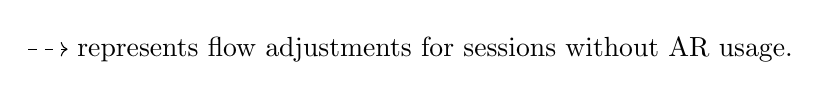
\begin{tikzpicture}[scale=0.5]
                \draw[->, dashed] (3,0) -- (4,0) node[right] {represents flow adjustments for sessions without AR usage.};
            \end{tikzpicture}\vspace{6pt}
        
    \caption{Flowchart of a session}
    \label{fig:experiment_flow}
\end{figure}

\subsection*{4. Expected Compensation}
% On average, students must earn at least what they are paid as student assistants by TUM.
The students will receive a fixed payment of 21€ for their participation, supplemented by an additional performance based payment. A participant can earn up to 15€ in addition to the fixed payment. The expected compensation for a participant is 29€. The experiment sessions will be overbooked to have enough participants even if some did not show up. The student that comes first will enter the experiment first. The students will be compensated with a show-up fee of 5€ if they were invited, and arrived on time but are not allowed to attend. All payments will be made in cash provided that the participant completes, and submits a compensation form with their last name, first name, date of birth, german tax ID, and address. These information is required as per TUM regulations for cash payments.

\subsection*{5. Anonymity and Data Protection}
Participants will connect via video conferencing for augmented reality (AR) sessions, during which dyad members will see each other and each other's perspectives on their computers and holographic screens. No conversations between the technician-expert dyad will be recorded, nor will any video footage be captured.

Performance data will be recorded manually and stored locally on the experimenter's laptop during the experiments. At the conclusion of the experiment, all participants will complete a questionnaire. Personal information such as names or matriculation numbers will not be collected. Instead, participants will be assigned unique identifiers during the experimentation process. This limits us in connecting the results of the experiment to an individual. 

The data obtained from the experiment and survey will be used for statistical analysis. The data will be stored on the experimenter's computer in a secured folder to prevent unauthorized access. The data may be stored and subjected to specific analyses for up to 10 years to facilitate further detailed analysis. Any additional analyses may be conducted by potential co-authors, but such analyses will be performed on anonymized data, which will remain password protected.

\subsection*{6. Anticipated Challenges}
We will use Microsoft HoloLens 2, an optical see-through head-mounted display. The advantage of using optical see-through display technology is that it allows participants to perceive the world as if they were wearing a normal pair of glasses. The HoloLens 2 features eye tracking and can adjust the holographic projection to accommodate different visual impairments. Additionally, it supports individuals who wear glasses, which reduces the likelihood of motion sickness commonly associated with virtual reality devices. A study involving 142 subjects found that the HoloLens induces negligible symptoms of simulator sickness.\footnote{Vovk, A., Wild, F., Guest, W., \& Kuula, T. (2018, April). Simulator sickness in augmented reality training using the Microsoft HoloLens. In \textit{Proceedings of the 2018 CHI conference on human factors in computing systems} (pp. 1-9).\\}

In our experiments, participants will be given instructions on a virtual reality device at the beginning of the experiment and report any motion sickness before beginning the experiment. Based on our extensive experience with virtual reality, participants usually know if they are prone to motion sickness. If not, they typically determine this within the first 5 minutes of use. Therefore, we anticipate that participants will be able to assess their ability to take part in the experiment after a 5-minute trial.

If students still witness physical drawbacks due to motion sickness or other adverse side effects, they may choose to terminate the trial. Students who drop out due to health issues will still be compensated for their participation (with the base pay but no performance-dependent payment).

The post-experiment questionnaire will also include questions regarding motion sickness and any difficulties experienced while using the AR headsets, which will be assessed on a Likert scale.

\subsection*{7. Exclusion Criteria}
\begin{enumerate}
\item 
Motion Sickness: Participants should not have a known history of motion sickness.

\item 
AR/VR Discomfort: Participants who experience discomfort (e.g., headaches, nausea) when using virtual reality or augmented reality devices.\footnote{If a participant is unaware of discomfort issues with AR and VR devices, and reports experiencing motion sickness during the introduction phase, they will be assigned the role of the expert, as the expert does not wear the AR glasses.}

\item 
Language: Participants who are unable to communicate in and understand English.
\end{enumerate}

\subsection*{8. Inclusion Criteria}
\begin{enumerate}
\item 
Age: Participants must be 18 years or older.

\item 
Health status: Participants must be healthy individuals without any medical conditions related to motion sickness that could be aggravated by participation in the study. 

\item 
Language: Participants must be able to communicate in and understand English.

\item 
Consent: Participants must sign informed consent to participate in the study.

\item 
Compensation Form: Participants must complete and send the consent form to participate in the study.
\end{enumerate}

\end{document}

 